% THIS IS AN EXAMPLE DOCUMENT FOR VLDB 2012
% based on ACM SIGPROC-SP.TEX VERSION 2.7
% Modified by  Gerald Weber <gerald@cs.auckland.ac.nz>
% Removed the requirement to include *bbl file in here. (AhmetSacan, Sep2012)
% Fixed the equation on page 3 to prevent line overflow. (AhmetSacan, Sep2012)

\documentclass{vldb}
\usepackage{graphicx}
\usepackage{balance}  % for  \balance command ON LAST PAGE  (only there!)
\usepackage[utf8x]{inputenc}
\usepackage[colorinlistoftodos]{todonotes}
\usepackage{adjustbox}
\usepackage{hyperref}
\usepackage{microtype}
\usepackage{pgfplots} % LaTeX
\usepgfplotslibrary{groupplots}

%%%%%%%%%%%%%%%%%%%%%%%%%%%%%%%%%%%%%
%usepackage{pgf}
\usepackage{tikz}
\usepackage{listings}
%%%<
\usepackage{verbatim}
%\usepackage[active,tightpage]{preview}
%\PreviewEnvironment{tikzpicture}
%\setlength\PreviewBorder{5pt}%
%%%>

%\usepackage[utf8]{inputenc}
\usetikzlibrary{arrows,automata}
%%%%%%%%%%%%%%%%%%%%%%%%%%%%%%%%%%%%%
\pgfplotsset{compat=1.11}




% Include information below and uncomment for camera ready
%\vldbTitle{Twitter data serialization methods and benchmarks}
\vldbTitle{Complex Object Implementations for Big Data Systems}
\vldbAuthors{Ben Trovato, G. K. M. Tobin, Lars Th{\sf{\o}}rv{$\ddot{\mbox{a}}$}ld, Lawrence P. Leipuner, Sean Fogarty, Charles Palmer, John Smith, Julius P.~Kumquat, and Ahmet Sacan}
\vldbDOI{https://doi.org/10.14778/xxxxxxx.xxxxxxx}
\vldbVolume{12}
\vldbNumber{xxx}
\vldbYear{2019}


\tikzset{
	state/.style={
		rectangle,
		rounded corners,
		draw=black, very thick,
		minimum height=2em,
		inner sep=2pt,
		text centered,
	},
	connect/.style = {  black },
}
\newcommand{\definevariableobject}[1] {\textcolor{black}{ 
		\ttfamily\bfseries\textcolor{red}{\ #1}}
} 
\newcommand{\definevariable}[1] {\textcolor{black}{ 
		\ttfamily\bfseries\ #1}
} 
\definecolor{copper}{cmyk}{0,0.9,0.9,0.2}
\colorlet{lightgray}{black!25}
\colorlet{darkgray}{black!75}

\begin{document}

% ****************** TITLE ****************************************

\title{Complex Object Implementations for Big Data Systems}


% possible, but not really needed or used for PVLDB:
%\subtitle{[Extended Abstract]
%\titlenote{A full version of this paper is available as\textit{Author's Guide to Preparing ACM SIG Proceedings Using \LaTeX$2_\epsilon$\ and BibTeX} at \texttt{www.acm.org/eaddress.htm}}}

% ****************** AUTHORS **************************************

% You need the command \numberofauthors to handle the 'placement
% and alignment' of the authors beneath the title.
%
% For aesthetic reasons, we recommend 'three authors at a time'
% i.e. three 'name/affiliation blocks' be placed beneath the title.
%
% NOTE: You are NOT restricted in how many 'rows' of
% "name/affiliations" may appear. We just ask that you restrict
% the number of 'columns' to three.
%
% Because of the available 'opening page real-estate'
% we ask you to refrain from putting more than six authors
% (two rows with three columns) beneath the article title.
% More than six makes the first-page appear very cluttered indeed.
%
% Use the \alignauthor commands to handle the names
% and affiliations for an 'aesthetic maximum' of six authors.
% Add names, affiliations, addresses for
% the seventh etc. author(s) as the argument for the
% \additionalauthors command.
% These 'additional authors' will be output/set for you
% without further effort on your part as the last section in
% the body of your article BEFORE References or any Appendices.

\numberofauthors{3} %  in this sample file, there are a *total*
% of EIGHT authors. SIX appear on the 'first-page' (for formatting
% reasons) and the remaining two appear in the \additionalauthors section.

\author{
% You can go ahead and credit any number of authors here,
% e.g. one 'row of three' or two rows (consisting of one row of three
% and a second row of one, two or three).
%
% The command \alignauthor (no curly braces needed) should
% precede each author name, affiliation/snail-mail address and
% e-mail address. Additionally, tag each line of
% affiliation/address with \affaddr, and tag the
% e-mail address with \email.
%
% 1st. author
\alignauthor
Saeed Fathollahzadeh \\
\affaddr{Free University of Bozen-Bolzano}\\
%\affaddr{P.O. Box 1212}\\
%\affaddr{Dublin, Ohio 43017-6221}\\
\email{saeed.fathollahzadeh@unibz.it}
% 2nd. author

\alignauthor
Kia Teymourian \\
\affaddr{Boston University}\\
%\affaddr{1932 Wallamaloo Lane}\\
%\affaddr{Wallamaloo, New Zealand}\\
\email{kiat@bu.edu}
% 3rd. author
\alignauthor 
	  Chris Jermaine \\
       \affaddr{Rice University}\\
       %\affaddr{1 Th{\large{\sf{\o}}}rv{$\ddot{\mbox{a}}$}ld Circle}\\
       %\affaddr{Hekla, Iceland}\\
       \email{cmj4@rice.edu}

}
% There's nothing stopping you putting the seventh, eighth, etc.
% author on the opening page (as the 'third row') but we ask,
% for aesthetic reasons that you place these 'additional authors'
% in the \additional authors block, viz.
\additionalauthors{Additional authors: John Smith (The Th{\o}rv\"{a}ld Group, {\texttt{jsmith@affiliation.org}}), Julius P.~Kumquat
(The \raggedright{Kumquat} Consortium, {\small \texttt{jpkumquat@consortium.net}}), and Ahmet Sacan (Drexel University, {\small \texttt{ahmetdevel@gmail.com}})}
\date{30 July 1999}
% Just remember to make sure that the TOTAL number of authors
% is the number that will appear on the first page PLUS the
% number that will appear in the \additionalauthors section.


\maketitle


\begin{abstract}
\todo[inline]{abstract}
\end{abstract}
\section{Introduction}
\todo[inline]{Introduction}
The contribution of our work are the following:
\begin{enumerate}
	\item we implement all serialization methods in C++ and Java programming language in a single thread system. But, we evaluate the methods with $task set$ for restrict run the method on a special core and without $task set$ to allow run method on the arbitrary cores. In the experimental section we mention which methods use thread or which platforms want to improve performance of processing.
	
	\item we implement same method in both C++ and Java programming language and we demonstrated same technique haven't same performance in differ languages(e.g, google protobuf).
	
	\item we compare all methods with a complex data sets. In academic setting over the last decade, there has been significant progress in serialization methods. However, much of this work makes assumptions that are simply unrealistic for deployed industrial applications. In this work, we used twitter dataset. This dataset include more objects type with deep hierarchy. Some methods need to save object meta data in serialization step and will be use it in the de-serialization section.    
	
	\item we investigate which methods are easy to used. It means is which methods create transparent view in develop step. For example in C++ $InPlace$ we need just one line for de-serialization, But in the serialization step we should spend more times for convert object to the method schema.
	
		
	\item we evaluate multiple famous serialization methods in big data systems. We focused specially on C++ and Java programming language. So, we deeply compared CPU, Memory and I/O for HDD resources. Our empirical experiments demonstrate best way for choose best method in a big data system.
	
	
\end{enumerate}
\section{Experimental Overview}

In the next few sections of the paper, we will give detailed explanations of the experimental tasks we consider. As a preview, the tasks we consider are:

\begin{figure*}[t]
	\centering
	\resizebox{!}{3.5in}{
	   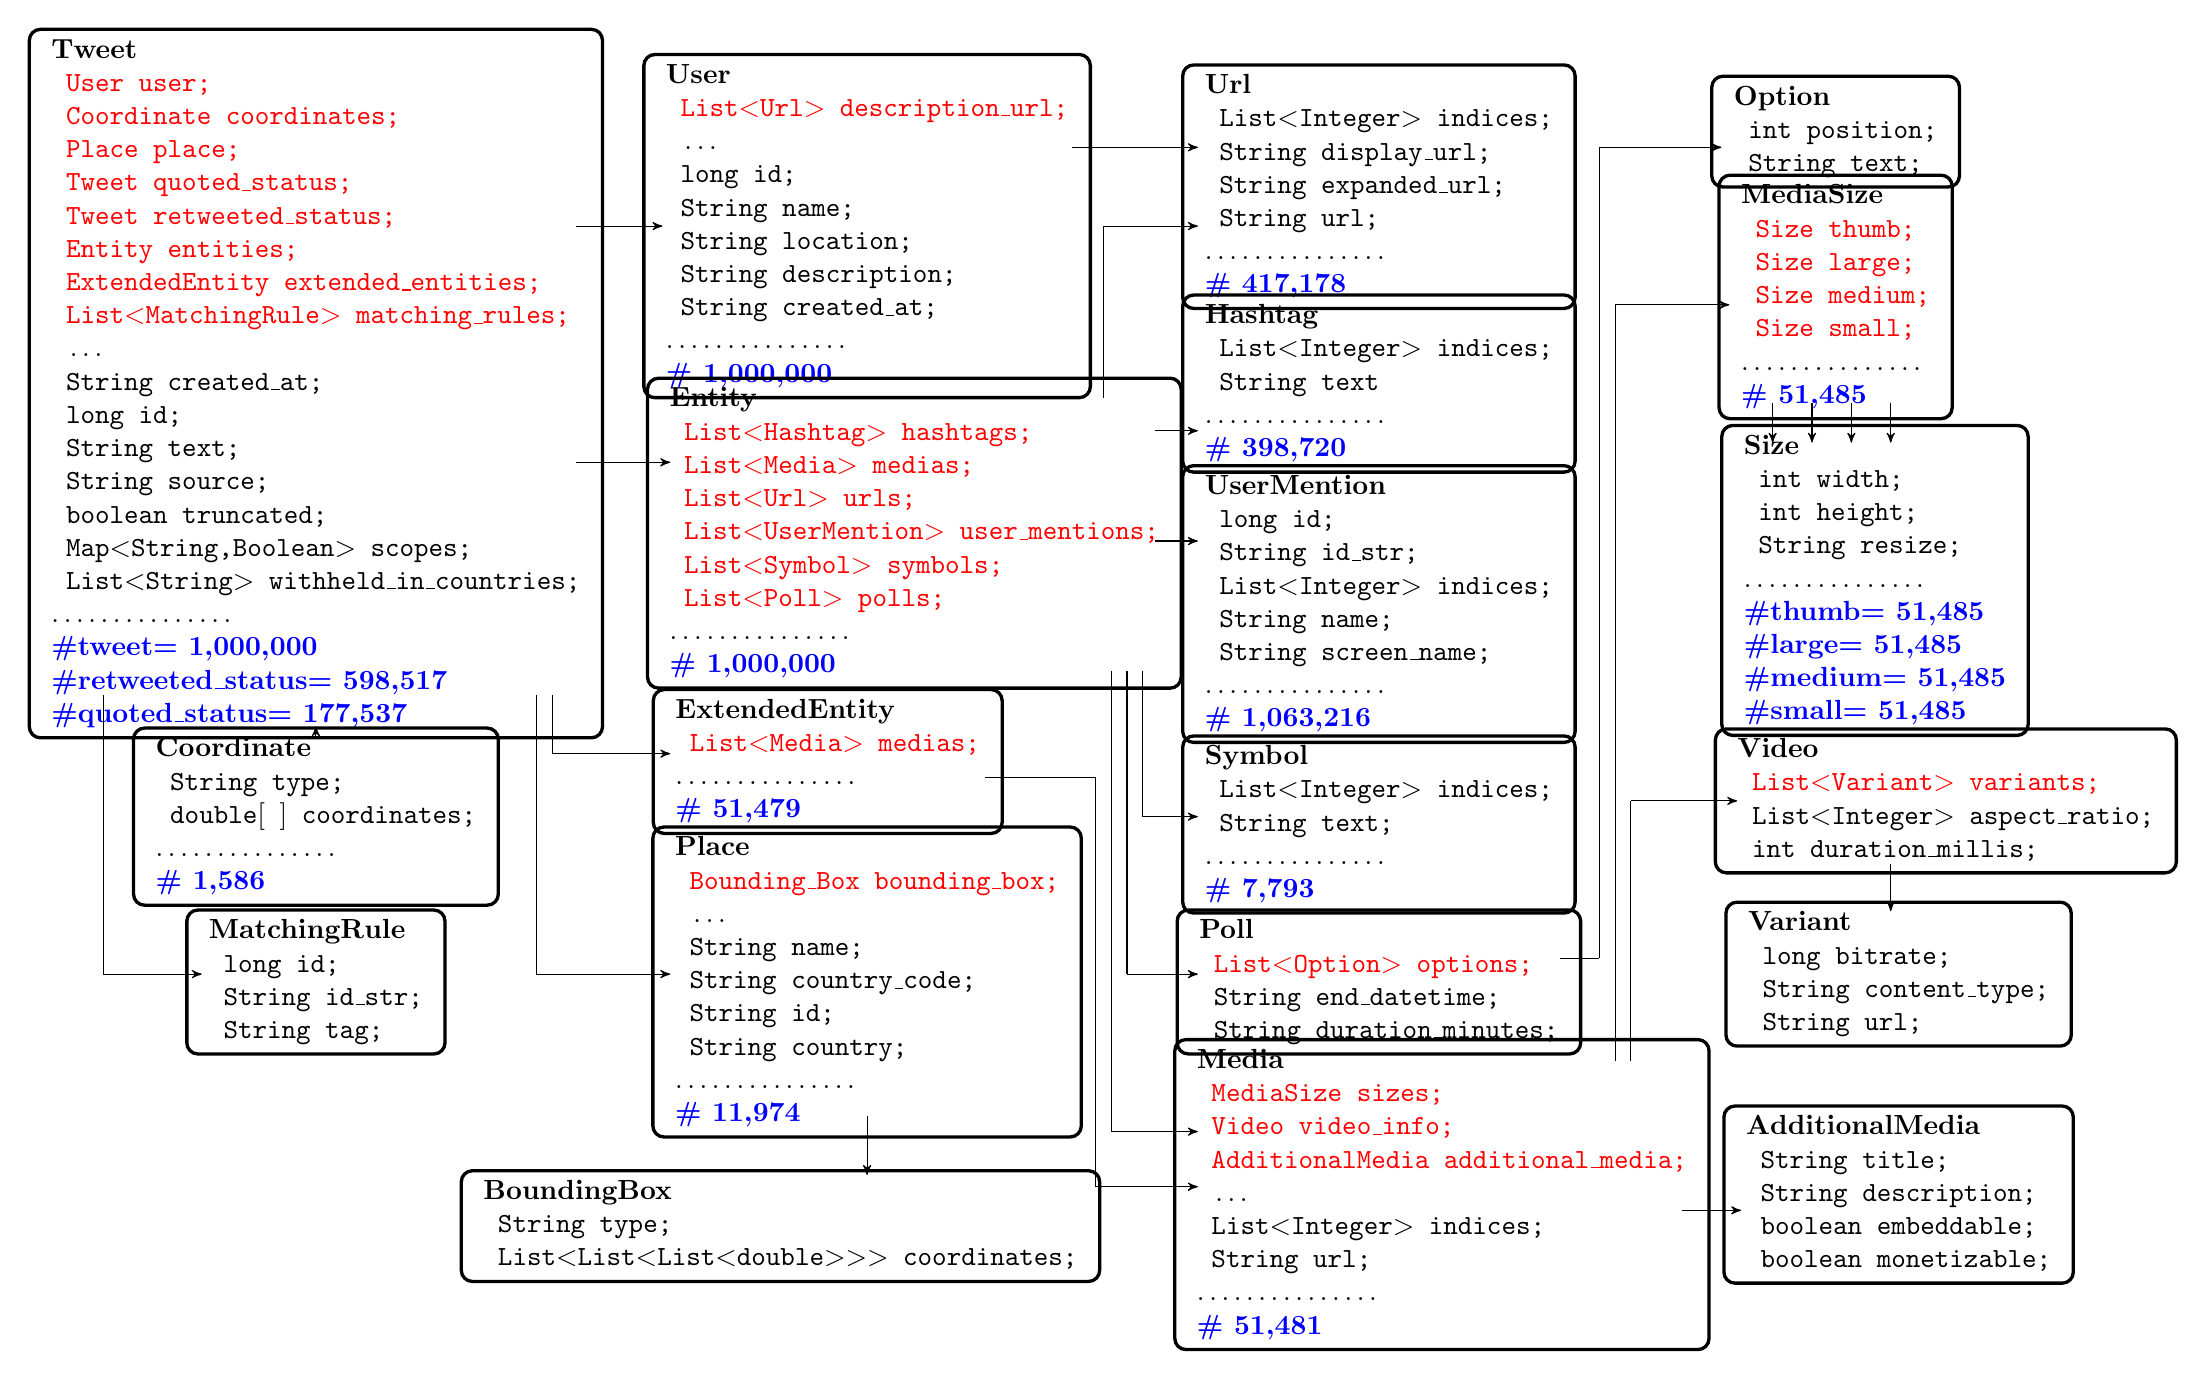
\begin{tikzpicture}[->,>=stealth']
\node[state] (TWEET) 
{\begin{tabular}{l}
	\textbf{Tweet}\\
	\definevariableobject{User user;}\\
	\definevariableobject{Coordinate coordinates;}\\
	\definevariableobject{Place place;}\\
	\definevariableobject{Tweet quoted\_status;}\\
	\definevariableobject{Tweet retweeted\_status;}\\
	\definevariableobject{Entity entities;}\\
	\definevariableobject{ExtendedEntity extended\_entities;}\\
	\definevariableobject{List$\textless$MatchingRule$\textgreater$ matching\_rules;}\\
	\ \  \ldots \\
	\definevariable{String created\_at;}\\
	\definevariable{long id;}\\
	\definevariable{String text;}\\
	\definevariable{String source;}\\
	\definevariable{boolean truncated;}\\
	\definevariable{Map$<$String,Boolean$>$ scopes;}\\
	\definevariable{List$<$String$>$ withheld\_in\_countries;}\\
	\ldots  \ldots  \ldots \ldots  \ldots \\
	\textcolor{blue}{\textbf{\#tweet= 1,000,000}}\\
	\textcolor{blue}{\textbf{\#retweeted\_status= 598,517}}\\
	\textcolor{blue}{\textbf{\#quoted\_status= 177,537}}\\
	\end{tabular}};

% Next node: User
\node[state,       
node distance=7cm,    
%text width=3cm,       
right of=TWEET,        
yshift=2cm] (USER)   
{                    
	\begin{tabular}{l}  
	\textbf{User}\\
	\definevariableobject{List$<$Url$>$ description\_url;}\\
	\ \  \ldots \\
	\definevariable{long id;}\\
	\definevariable{String name;}\\
	\definevariable{String location;}\\
	\definevariable{String description;}\\
	\definevariable{String created\_at;}\\
	\ldots  \ldots  \ldots \ldots  \ldots \\
	\textcolor{blue}{\textbf{\# 1,000,000}}\\
	\end{tabular}
};

% Next node: Coordinates
\node[state, yshift=-5.5cm] (COORDINATE) 
{
	\begin{tabular}{l}   
	\textbf{Coordinate}\\
	\definevariable{String type;}\\
	\definevariable{double$[\ ]$ coordinates;}\\
	\ldots  \ldots  \ldots \ldots  \ldots \\
	\textcolor{blue}{\textbf{\# 1,586}}\\
	\end{tabular}
};
% Next node: MatchingRule
\node[state, yshift=-7.6cm](MatchingRule)
{                    
	\begin{tabular}{l}   
	\textbf{MatchingRule}\\
	\definevariable{long id;}\\
	\definevariable{String id\_str;}\\
	\definevariable{String tag;}\\
	% \ldots  \ldots  \ldots \ldots  \ldots \\
	%\textcolor{blue}{\textbf{\# 1,586}}\\
	\end{tabular}
};

% Next node: Coordinates
\node[state,
node distance=7.6cm,    
%text width=3cm,       
right of=TWEET,        
yshift=+-1.9cm] (ENTITY)    
{%                    
	\begin{tabular}{l}     
	\textbf{Entity}\\
	\definevariableobject{List$<$Hashtag$>$ hashtags;}\\
	\definevariableobject{List$<$Media$>$ medias;}\\
	\definevariableobject{List$<$Url$>$ urls;}\\
	\definevariableobject{List$<$UserMention$>$ user\_mentions;}\\
	\definevariableobject{List$<$Symbol$>$ symbols;}\\
	\definevariableobject{List$<$Poll$>$ polls;}\\
	\ldots  \ldots  \ldots \ldots  \ldots \\
	\textcolor{blue}{\textbf{\# 1,000,000}}\\
	\end{tabular}
};
% Next node: ExtendedEntity
\node[state,      
node distance=6.5cm,     
%text width=3cm,        
right of=TWEET,        
yshift=+-4.8cm] (EXTENDEDENTITY)    
{%                     
	\begin{tabular}{l}     
	\textbf{ExtendedEntity}\\
	\definevariableobject{List$<$Media$>$ medias;}\\
	\ldots  \ldots  \ldots \ldots  \ldots \\
	\textcolor{blue}{\textbf{\# 51,479}}\\
	\end{tabular}
};

% Next node: Place
\node[state,       
node distance=7cm,     
%text width=3cm,        
right of=TWEET,       
yshift=+-7.6cm] (PLACE)    
{%                    
	\begin{tabular}{l}     
	\textbf{Place}\\
	\definevariableobject{Bounding\_Box bounding\_box;}\\
	\ \  \ldots \\
	\definevariable{String name;}\\
	\definevariable{String country\_code;}\\
	\definevariable{String id;}\\
	\definevariable{String country;}\\
	\ldots  \ldots  \ldots \ldots  \ldots \\
	\textcolor{blue}{\textbf{\# 11,974}}\\
	
	\end{tabular}
};

% Next node: BoundingBoxCoordinate
\node[state,       
node distance=5.9cm,     
%text width=3cm,        
right of=TWEET,        
yshift=-10.7cm] (BoundingBoxCoordinate)    
{%                     
	\begin{tabular}{l}     
	\textbf{BoundingBox}\\	
	\definevariable{String type;}\\
	\definevariable{List$<$List$<$List$<$double$>>>$ coordinates;}\\	
	%\ldots  \ldots  \ldots \ldots  \ldots \\
	%\textcolor{blue}{\textbf{\# 11,974}}\\	
	\end{tabular}
};

private String type;
private List<List<List<Double>>> coordinates;

% Next node: Urls
\node[state,       
node distance=6.5cm,    
right of=USER,       
yshift=0.5cm] (URL)   
{
	\begin{tabular}{l}    
	\textbf{Url}\\
	\definevariable{List$<$Integer$>$ indices;}\\
	\definevariable{String display\_url;}\\
	\definevariable{String expanded\_url;}\\
	\definevariable{String url;}\\
	\ldots  \ldots  \ldots \ldots  \ldots \\
	\textcolor{blue}{\textbf{\# 417,178}}\\
	
	\end{tabular}
};

% Next node: Hashtag
\node[state,       
node distance=6.5cm,    
right of=USER,       
yshift=-2cm] (HASHTAG)   
{
	\begin{tabular}{l}    
	\textbf{Hashtag}\\
	\definevariable{List$<$Integer$>$ indices;}\\
	\definevariable{String text}\\	
	\ldots  \ldots  \ldots \ldots  \ldots \\
	\textcolor{blue}{\textbf{\# 398,720}}\\
	\end{tabular}	
};

% Next node: Hashtag
\node[state,       
node distance=6.5cm,    
right of=USER,       
yshift=-4.8cm] (USERMENTION)   
{
	\begin{tabular}{l}    
	\textbf{UserMention}\\
	\definevariable{long id;}\\
	\definevariable{String id\_str;}\\
	\definevariable{List$<$Integer$>$ indices;}\\
	\definevariable{String name;}\\
	\definevariable{String screen\_name;}\\	
	\ldots  \ldots  \ldots \ldots  \ldots \\
	\textcolor{blue}{\textbf{\# 1,063,216}}\\
	\end{tabular}	
};

% Next node: Symbol
\node[state,       
node distance=6.5cm,    
right of=USER,       
yshift=-7.6cm] (SYMBOL)   
{
	\begin{tabular}{l}    
	\textbf{Symbol}\\	
	\definevariable{List$<$Integer$>$ indices;}\\
	\definevariable{String text;}\\	
	\ldots  \ldots  \ldots \ldots  \ldots \\
	\textcolor{blue}{\textbf{\# 7,793}}\\
	\end{tabular}	
};

% Next node: Poll
\node[state,       
node distance=6.5cm,    
right of=USER,       
yshift=-9.6cm] (POLL)   
{
	\begin{tabular}{l}    
	\textbf{Poll}\\	
	\definevariableobject{List$<$Option$>$ options;}\\
	\definevariable{String end\_datetime;}\\	
	\definevariable{String duration\_minutes;}\\	
	%\ldots  \ldots  \ldots \ldots  \ldots \\
	%\textcolor{blue}{\textbf{\# 7,793}}\\
	\end{tabular}	
};
% Next node: Media
\node[state,       
node distance=7.3cm,    
right of=USER,       
yshift=-12.3cm] (MEDIA)   
{
	\begin{tabular}{l}    
	\textbf{Media}\\	
	\definevariableobject{MediaSize sizes;}\\
	\definevariableobject{Video video\_info;}\\
	\definevariableobject{AdditionalMedia additional\_media;}\\
	\ \  \ldots \\
	\definevariable{List$<$Integer$>$ indices;}\\
	\definevariable{String url;}\\
	\ldots  \ldots  \ldots \ldots  \ldots \\
	\textcolor{blue}{\textbf{\# 51,481}}\\
	\end{tabular}	
};

% Next node: Media
\node[state,       
node distance=5.8cm,    
right of=URL,       
yshift=0.7cm] (OPTION)   
{
	\begin{tabular}{l}    
	\textbf{Option}\\		
	\definevariable{int position;}\\
	\definevariable{String text;}\\
	%\ldots  \ldots  \ldots \ldots  \ldots \\
	%\textcolor{blue}{\textbf{\# 51,481}}\\
	\end{tabular}	
};

% Next node: MediaSize
\node[state,       
node distance=2cm,    
below of=OPTION,       
yshift=-0.1cm] (MEDIASIZA)   
{
	\begin{tabular}{l}    
	\textbf{MediaSize}\\		
	\definevariableobject{Size thumb;}\\
	\definevariableobject{Size large;}\\
	\definevariableobject{Size medium;}\\
	\definevariableobject{Size small;}\\
	\ldots  \ldots  \ldots \ldots  \ldots \\
	\textcolor{blue}{\textbf{\# 51,485}}\\
	\end{tabular}	
};

% Next node: Size
\node[state,       
node distance=6.3cm,    
right of=USERMENTION,       
yshift=0.3cm] (SIZE)   
{
	\begin{tabular}{l}    
	\textbf{Size}\\		
	\definevariable{int width;}\\
	\definevariable{int height;}\\
	\definevariable{String resize;}\\
	
	\ldots  \ldots  \ldots \ldots  \ldots \\
	\textcolor{blue}{\textbf{\#thumb= 51,485}}\\
	\textcolor{blue}{\textbf{\#large= 51,485}}\\
	\textcolor{blue}{\textbf{\#medium= 51,485}}\\
	\textcolor{blue}{\textbf{\#small= 51,485}}\\
	\end{tabular}	
};

% Next node: Video
\node[state,       
node distance=7.2cm,    
right of=SYMBOL,       
yshift=0.3cm] (VIDEO)   
{
	\begin{tabular}{l}    
	\textbf{Video}\\		
	\definevariableobject{List$<$Variant$>$ variants;}\\
	\definevariable{List$<$Integer$>$ aspect\_ratio;}\\
	\definevariable{int duration\_millis;}\\
	
	%\ldots  \ldots  \ldots \ldots  \ldots \\
	%\textcolor{blue}{\textbf{\#thumb= 51,485}}\\
	
	\end{tabular}	
};
% Next node: Variant
\node[state,       
node distance=6.6cm,    
right of=SYMBOL,       
yshift=-1.9cm] (Variant)   
{
	\begin{tabular}{l}    
	\textbf{Variant}\\		
	\definevariable{long bitrate;}\\
	\definevariable{String content\_type;}\\
	\definevariable{String url;}\\
	
	%\ldots  \ldots  \ldots \ldots  \ldots \\
	%\textcolor{blue}{\textbf{\#thumb= 51,485}}\\
	
	\end{tabular}	
};

% Next node: AdditionalMedia
\node[state,       
node distance=5.8cm,    
right of=MEDIA,       
yshift=0cm] (AdditionalMedia)   
{
	\begin{tabular}{l}    
	\textbf{AdditionalMedia}\\		
	\definevariable{String title;}\\
	\definevariable{String description;}\\
	\definevariable{boolean embeddable;}\\
	\definevariable{boolean monetizable;}\\	
	%\ldots  \ldots  \ldots \ldots  \ldots \\
	%\textcolor{blue}{\textbf{\#thumb= 51,485}}\\
	
	\end{tabular}	
};

\draw[connect] (3.3,2) -- (4.4,2) ;% TWEET -> User
\draw[connect] (3.3,-1) -- (4.5,-1) ;% TWEET -> User
\draw[connect] (3, -3.95) -- (3,-4.7) (3,-4.7) -- (4.5,-4.7) ;% TWEET -> Extended Entity
\draw[connect] (2.8, -3.95) -- (2.8,-7.5) (2.8,-7.5) -- (4.5,-7.5) ; % TWEEt -> Place
\draw[connect] (-2.7, -3.95) -- (-2.7,-7.5) (-2.7,-7.5) -- (-1.45,-7.5) ; % TWEEt -> Matching Rules
\draw[connect] (9.6,3) -- (11.2,3) ;% User -> Url
\draw[connect] (10,2)  -- (10,-0.18)  (10,2) -- (11.2,2) ;% Entity -> Url
\draw[connect] (7,-9.3)  -- (7,-10.05) ;% Place -> BondBox
\draw[connect] (10.65,-0.6) -- (11.2,-0.6) ;% Entity -> Hashtag
\draw[connect] (10.65,-2) -- (11.2,-2) ;% Entity -> User Mention
\draw[connect] (10.5,-3.65)  -- (10.5,-5.5)  (10.5,-5.5) -- (11.2,-5.5) ;% Entity -> User Mention
\draw[connect] (10.3,-3.65)  -- (10.3,-7.5)  (10.3,-7.5) -- (11.2,-7.5) ;% Entity -> Poll
\draw[connect] (10.1,-3.65)  -- (10.1,-9.5)  (10.1,-9.5) -- (11.2,-9.5) ;% Entity -> Media
\draw[connect]  (8.5,-5) --(9.9,-5) (9.9,-5)  -- (9.9,-10.2)  (9.9,-10.2) -- (11.2,-10.2) ;%  Extend Entity -> Media
\draw[connect](15.8,-7.3) -- (16.3,-7.3) (16.3,3)  -- (16.3,-7.3)  (16.3,3) -- (17.85,3) ;% Poll -> Option
\draw[connect] (16.5,1)  -- (16.5,-8.6)  (16.5,1) -- (17.95,1) ;% Media -> Media Size
\draw[connect] (16.7,-5.3)  -- (16.7,-8.6)  (16.7,-5.3) -- (18.05,-5.3) ;% Media -> Video
\draw[connect] (17.35,-10.5) -- (18.1,-10.5) ;% Media -> AdditionalMedia
\draw[connect] (18.5,-0.25)  -- (18.5,-0.75) ;% Media Size -> Size
\draw[connect] (19,-0.25)  -- (19,-0.75) ;% Media Size -> Size
\draw[connect] (19.5,-0.25)  -- (19.5,-0.75) ;% Media Size -> Size
\draw[connect] (20,-0.25)  -- (20,-0.75) ;% Media Size -> Size
\draw[connect] (20,-6.1)  -- (20,-6.7) ;% Media Size -> Size

\path %(TWEET) edge (USER)
(TWEET) edge (COORDINATE) ;
\end{tikzpicture}



	 }
	\caption{Object relationship and frequency of Tweet Objects (for one million tweets)}
	\label{fig:tweet_complex_object}
\end{figure*}

\begin{enumerate}
	\item A set of serialized objects stored externally on an HDD; the task is to read the objects into memory and deserialize them to their in-memory representation.
	\item A set of objects are stored in a large file (larger than the available RAM). The task is to perform an external sort of the file in order to perform a duplicate removal.
	\item A set of objects are partitioned across a number of machines in a network; the task is to send requests to the 	machines. Each machine answers the request by serializing the objects, then sending them over the network to the requesting machine.
	\item Finally, a set of sparse vectors are stored across various machines on a network. The task is to perform a tree aggregation where the vectors are aggregated over $log ( n )$
	hops.
\end{enumerate}

\subsection{Twitter Data Set}
For the various experiments, we use twitter data sets \cite{tweet_objects}, implemented using each of the ten different physical implementations. 

\subsection{Encoding sizes}
The ten different complex object implementations that we considered have very different encoding densities when the objects are serialized for storage or transmission across the network. The average, per-object sizes are given in Table %\ref{tbl:object_size}. 
%\begin{table}
%	\centering
%	\caption{Frequency of some Tweet Objects  (for 1 million tweets) }
%	\label{tbl:object_size}
%	\begin{adjustbox}{width=\columnwidth,center}	
		
%		\begin{tabular}{|c|c|c|} \hline
%			Object Name &Parent Object &Frequency\\ \hline
%			tweet  & root object& 1,000,000 \\ \hline
%			users & tweet & 1,000,000 \\ \hline
%			coordinates  &tweet& 1586 \\ \hline
%			place & tweet & 11974 \\ \hline
%			quoted status  & tweet & 177537 \\ \hline
%			retweeted status  & tweet & 598517 \\ \hline
%			entities  & tweet & 1,000,000 \\ \hline
%			extended entities  & tweet & 51479 \\ \hline
%			hashtags  & entities & 398720 \\ \hline
%			media  & entities & 51481 \\ \hline
%			urls  & entities & 417176 \\ \hline
%			user mentions  & entities & 1063216 \\ \hline
%			symbols  & entities & 7793 \\ \hline
%			sizes  & media & 7793 \\ \hline
%			media sizes  & sizes & 51485 \\ \hline
%			thumb  & media sizes & 51485 \\ \hline
%			large  & media sizes & 51485 \\ \hline
%			medium  & media sizes & 51485 \\ \hline
%			small  & media sizes & 51485 \\ \hline
%			\hline\end{tabular}
%	\end{adjustbox}
%\end{table}

\begin{table}
	\centering
	\caption{tweet complexity }
	\label{tbl:object_size}
	\begin{adjustbox}{width=\columnwidth,center}	
		
		\begin{tabular}{|c|c|} \hline
			Tweet type & Frequency\\ \hline
			Simple tweets(retweet \& quote are null ) & 332,901\\ \hline
			Retweets & 489,562\\ \hline
			Quote & 68,582\\ \hline
			Retweet \& Quote & 108,955\\ \hline
			Total & 1,000,000 \\ \hline
			
			\hline\end{tabular}
	\end{adjustbox}
\end{table}

\begin{table}
	\centering
	\caption{Comparison of object size for 1 million tweet }
	\label{tbl:object_size}
	\begin{adjustbox}{width=\columnwidth,center}	
		
		\begin{tabular}{|l|c|c|} \hline
		 \textbf{Serialization Methods} & \textbf{Serialized file size(gigabyte)}\\ \hline
			Java Default  & 4.6 \\ \hline	
			Java Json Gzip  & 1.4 \\ \hline	
			Java Bson  & 4.9 \\ \hline	
			Java Protocol Buffer  & 1.9 \\ \hline	
			Java Kyro  & 1.9 \\ \hline	
			Java Hand Coded ByteBuffer  & 2.3 \\ \hline	
			Java FaltBuffers  & 2.9 \\ \hline	
			C++ Hand Coded  & 2.1 \\ \hline	
			C++ InPlace  & 3.2 \\ \hline	
			C++ Boost  & 2.2 \\ \hline	
			C++ Protocol Buffer  & 1.9 \\ \hline
			C++ Bson  & 4.6 \\ \hline	
			C++ FaltBuffers  & 2.9 \\ \hline	
			Rust Json  & 4.8 \\ \hline
			Rust Bincode  & 2.4 \\ \hline			
			Rust MessagePack  & 1.9 \\ \hline			
			Rust Bson  & 4.5 \\ \hline			
			Rust FlexBuffers  & 4.3 \\ 						
			\hline\end{tabular}
	\end{adjustbox}
\end{table}

\begin{table}
	\centering
	\caption{Lines of code for serialization and de-serialization  }
	\label{tbl:object_size}
	\begin{adjustbox}{width=\columnwidth,center}	
		
		\begin{tabular}{|l|c|c|} \hline
			\textbf{Serialization Methods} & \textbf{Serialize} &  \textbf{De-Serialize}   \\ \hline
			Java Default  & 4  & 4 \\ \hline	
			Java Json Gzip  & 2 & 4\\ \hline	
			Java Bson  & 50  & 120 \\ \hline	
			Java Protocol Buffer  & 200 & 1 \\ 
			                      &\textcolor{red}{with 20 extra files} &  \\ \hline	
			Java Kyro  & 40 & 40 \\ \hline	
			Java Hand Coded ByteBuffer  & 150 & 150 \\ \hline	
			Java FaltBuffers  & 250 & 1 \\ 
							  &\textcolor{red}{with 42 extra files} &  \\ \hline	
			C++ Hand Coded  & 70  & 100 \\ \hline	
			C++ InPlace  & 80 & 1 \\ \hline	
			C++ Boost  & 1 & 2 \\ \hline	
			C++ Protocol Buffer  & 200 & 1\\ 
									&\textcolor{red}{with 20 extra files} &  \\ \hline	
			C++ Bson  & 40 & 100 \\ \hline	
			C++ FaltBuffers  & 250  & 1 \\ 
									&\textcolor{red}{with 42 extra files} &  \\ 	\hline	
			Rust Json  & 1 & 1 \\ \hline
			Rust Bincode  & 1 & 1\\ \hline			
			Rust MessagePack  & 1 & 1\\ \hline			
			Rust Bson  & 1 & 1\\ \hline			
			Rust FlexBuffers  & 1 & 1\\						
			\hline\end{tabular}
	\end{adjustbox}
\end{table}




\subsection{Experimental Details}
We run our experiments on Google Cloud costume instances which have 4 vCPU cores, 32 GB RAM and 3000 GB standard persistent disk(Sustained random IOPS limit: read=2,250 and write=4,500) running with Ubuntu Ubuntu 18.04.4 LTS. Before running each experiment task, we "warmed up" the Java Garbage Collector (GC) by creating a large number of objects. We do not include this warm-up-time in our performance time calculations.

We used two Java GC flags $-XX:-UseGCOverheadLimit$ and $-XX:+UseConcMarkSweepGC$. The first flag is used to avoid OutOfMemoryError exceptions while using the complete RAM size for data processing and the second flag is for running concurrent garbage collection.

We run all of our experiments 3 times and observed that the results have low variance. In this paper we present the average of those runs. Before running each experiment, we deleted th OS cache using the Linux command: $echo 3 > /proc/sys/vm/drop\_caches$.

Our Java implementation is written using Java 8 with the Oracle JDK version "1.8.0\_241" and for our C++ implementation we use the C++11, compiled using clang++ (version 6.0.0).

The source codes of our implementation and a brief description of technical details can be found on the Github Repository \footnote{The source code of our Implementation is available at \url{https://github.com/fathollahzadeh/serialization}} .

\section{Experiments}

\subsection{Serialize RAW Data to Local Disk}

The first step of experiments are serialize various complex objects and the write into a file in disk. In this experiment, the raw tweet data set read line-by-line and convert to a objects. The serialization tasks for each of the thirteen implementation method run. In the serialization process each object serialized or copy the final serialization result into $256KB$ pages and the objects indexed in separate file.

%\begin{figure}[t]
%	\centering
%	\resizebox{\columnwidth}{1.5in}{
%		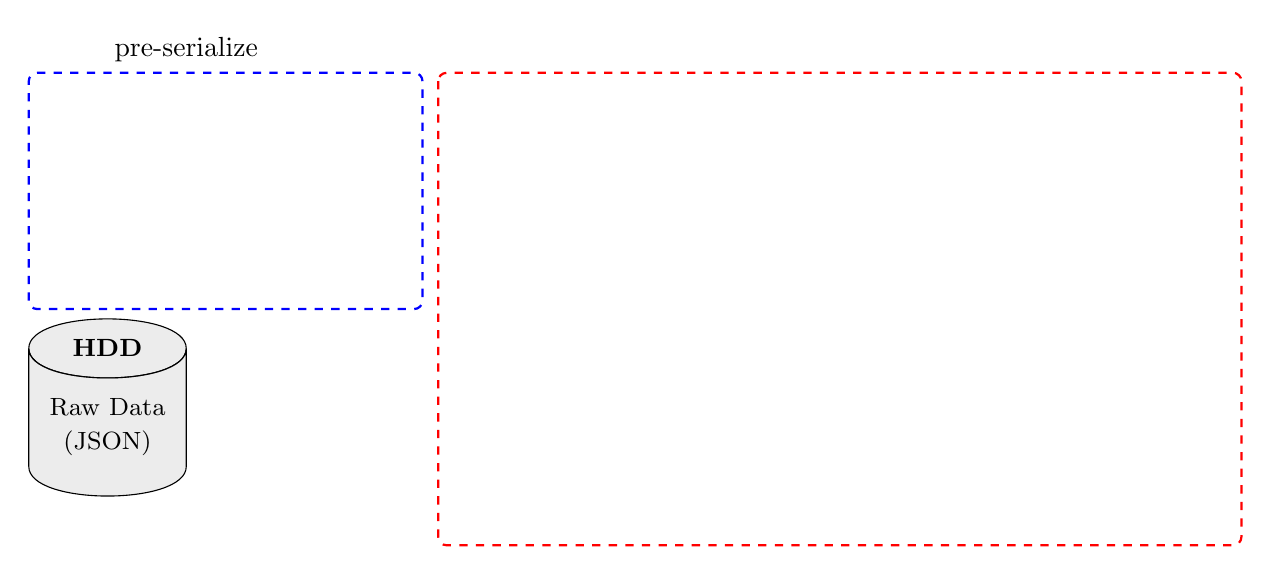
\begin{tikzpicture}
\draw (2,3.3) node{pre-serialize};
\draw[blue,thick,dashed,rounded corners=3pt](0,0) rectangle ++(5,3);
\draw[red,thick,dashed,rounded corners=3pt](5.2,3) rectangle ++(10.2,-6);

%\draw (0,0) -- (10,0) -- (10,4) -- (0,4) -- (0,0);

  \draw[fill=lightgray!60, fill opacity=0.5] (0,-0.5) to
 [controls=+(90:0.5) and +(90:0.5)] (2,-0.5);
 
 \draw[fill=lightgray!60, fill opacity=0.5] (0,-0.5) .. controls +(-90:0.5)
 and +(-90:0.5) .. (2,-0.5);
 
 \draw[fill=lightgray!60, fill opacity=0.5] (0,-0.5) .. controls +(-90:0.5)
 and +(-90:0.5) .. (2,-0.5)
 -- (2,-2) .. controls +(-90:0.5) and +(-90:0.5) .. (0,-2) -- (0,-0.5);
 
 \draw (1,-0.5) node[align=center,text width=1.5cm] {\centering\small\textbf{HDD}};
 \draw (1,-1.5) node[align=center,text width=1.5cm] {\centering\small{Raw Data (JSON)}};
 
 
 
\end{tikzpicture}
%	}
%	\caption{serialize process}
%	\label{fig:serialize_process}
%\end{figure} 

\begin{figure}
	\centering
	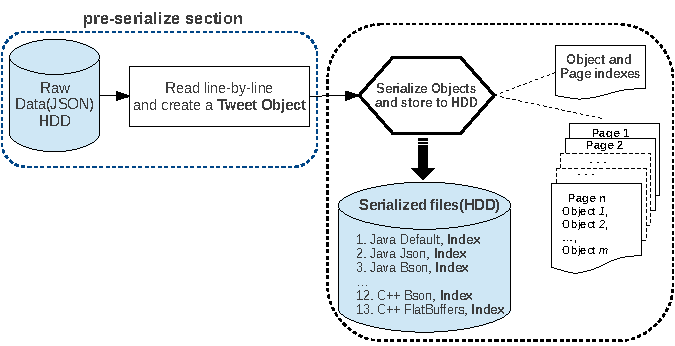
\includegraphics[width=\columnwidth,height=2.3in,keepaspectratio]{img/serialize_process.pdf}
	\caption{serialize process}
	\label{fig:serialize_process}
\end{figure}

\subsubsection{Results}

In Figure \ref{fig:exp_serialization_bar}, we show, for each of the thirteen implementations, for both $taskset$ TRUE and FALSE the total running time required as a function of the number of Tweet objects write experiments. In the figure where the
performance differences are easier to see; we also breakdown
the total time into I/O and CPU.
\begin{figure}
	\centering
	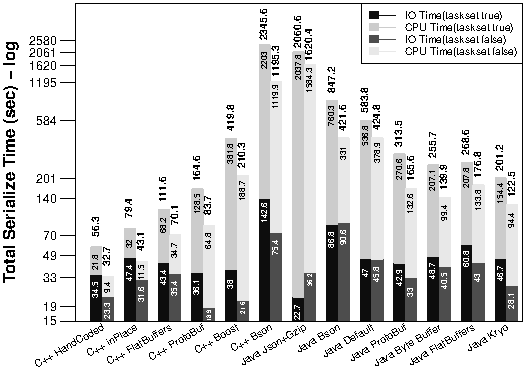
\includegraphics[width=\columnwidth,height=2.5in,keepaspectratio]{../../RScripts/Experiment_SerializeObjects_Bar.pdf}
	\caption{Serialize Objects for 5M Tweets}
	\label{fig:exp_serialization_bar}
\end{figure}

\subsubsection{Discussion}


\subsection{I/O FROM LOCAL DISK}
 The goal is to examine how the various complex object implementations compare for a simple from-disk retrieval task. In this set of experiments, the tweet data set is first loaded onto the HDD drive of a machine where they are organized into $256KB$ pages. The objects are then indexed, using a dense index.

Two experiments are run. In the first, a particular object is looked up in the index, and then enough pages are read from disk to access that object, as well as the following $n − 1$ objects. As the pages are loaded into RAM, all n objects are de-serialized and made ready for processing. This tests the ability of the object implementation to support fast processing of objects in sequence. We test $n$ in \{  $1\times 10^6$ , $2\times10^6$, $3\times10^6$, $4\times10^6$, $5\times10^6$ \}.

In the second experiment, a list of n, randomly-selected objects are accessed, in order. For each object, the location of the object in the database is looked up in the index, and then the corresponding page is loaded into RAM. The desired object is then de-serialized from the page. This simulates a scenario where objects are retrieved from secondary storage using a secondary index.

Before the experiment, the operating system buffer cache is emptied. We do not utilize a dedicated buffer cache, but we do allow the operating system to cache disk pages.

\subsubsection{Results}

\begin{figure}
	\centering
	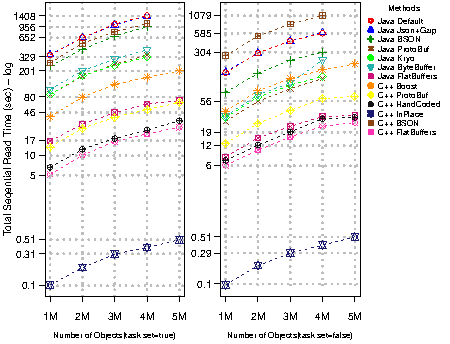
\includegraphics[width=\columnwidth,height=3in,keepaspectratio]{../../RScripts/Experiment_Seq_Read_CPU_Plot.pdf}
	\caption{sequential read}
	\label{fig:seq_read}
\end{figure}
\begin{figure}
	\centering
	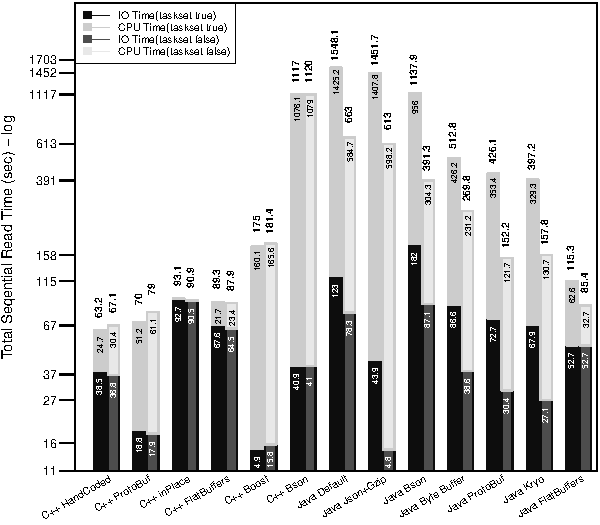
\includegraphics[width=\columnwidth,height=3in,keepaspectratio]{../../RScripts/Experiment_Seq_Read_CPU_IO_Bar.pdf}
	\caption{CPU and IO details of sequential read for 4M tweets}
	\label{fig:seq_read_detail}
\end{figure}

\begin{figure}
	\centering
	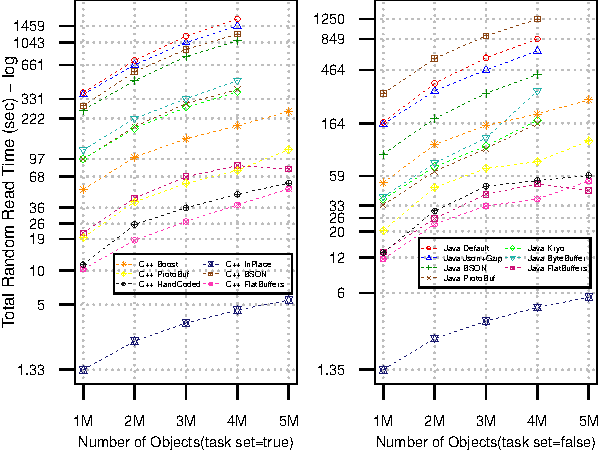
\includegraphics[width=\columnwidth,height=3in,keepaspectratio]{../../RScripts/Experiment_Rand_Read_CPU_Plot.pdf}
	\caption{random read}
	\label{fig:rand_read}
\end{figure}

\begin{figure}
	\centering
	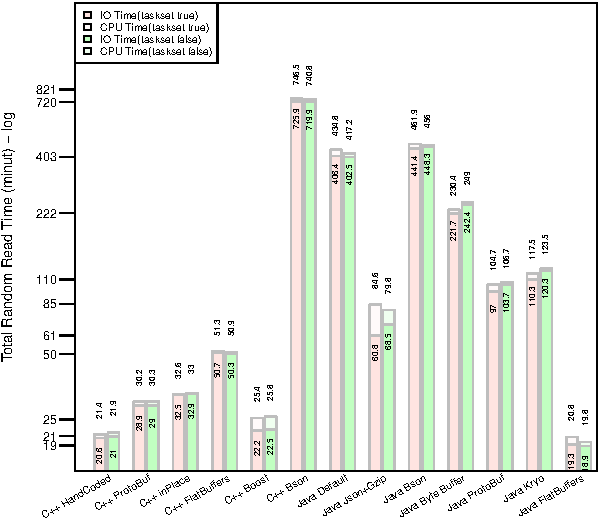
\includegraphics[width=\columnwidth,height=3in,keepaspectratio]{../../RScripts/Experiment_Rand_Read_CPU_IO_Bar.pdf}
	\caption{CPU and IO details of random read for 4M tweets}
	\label{fig:rand_read_detail}
\end{figure}

\subsubsection{Discussion}


\subsection{Exp. Memory usage}

\begin{figure}
	\centering
	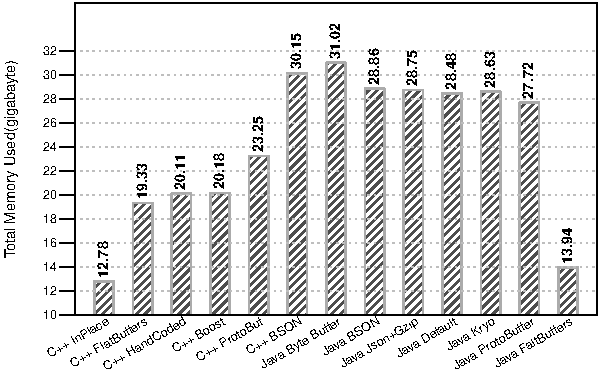
\includegraphics[width=\columnwidth,height=2.5in,keepaspectratio]{../../RScripts/Experiment_ReadObjects_Memory.pdf}
	\caption{memory used in read objects for 4M Tweets}
	\label{fig:exp_memory}
\end{figure}

\subsection{Exp. External Sort}
\begin{figure}
	\centering
	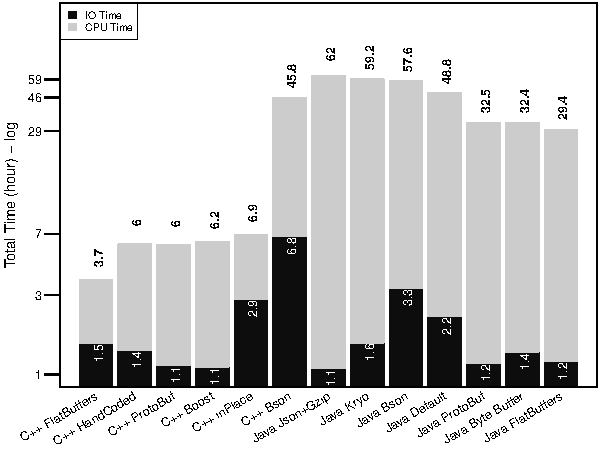
\includegraphics[width=\columnwidth,height=2in,keepaspectratio]{../../RScripts/Experiment_External_Sort_CPU_IO_Bar.pdf}
	\caption{external sort for 60M tweet}
	\label{fig:exp_memory}
\end{figure}



\bibliographystyle{abbrv}
\bibliography{References} 

\end{document}
